\begin{frame}
\frametitle{Mobility: motivación}
\begin{itemize}
\item<1-> La \textit{mobilidad} en ajedrez es una medida de la cantidad de movimientos que puede hacer un jugador en una posición.
\item<2-> Un paper de Eliot Slater (1950) mostró que hay una correlación entre la mobilidad de un jugador y la cantidad de partidas ganadas.
\item<3-> Se usa en funciones de evaluación hechas a mano.
\item<4-> Propongo agregar mobilidad como features en la red.
\end{itemize}
\end{frame}

\begin{frame}
\frametitle{Mobility: experimento}
Hay dos maneras de codificar la mobilidad:
\begin{itemize}
\item Bitsets (por rol/color)
\item Cantidades (por rol/color)
\end{itemize}
\end{frame}

\begin{frame}
\frametitle{Mobility: experimento (bitsets)}
Los features proveen \textbf{las celdas} a las que una pieza de determinado rol/color puede moverse.
\begin{figure}[H]
\begin{adjustbox}{max width=\textwidth}
\centering
\begin{tabular}{ccccc}
\raisebox{-7ex}{\chessboard[
    clearboard,
    setfen=r5k1/1b1p1ppp/p7/1p1Q4/2p1r3/PP4Pq/BBP2b1P/R4R1K w - - 0 20,
    tinyboard,
    showmover=false,
]}
&

\raisebox{-7ex}{\chessboard[
    tinyboard,
    clearboard,
    showmover=false,
    setwhite={ba2,bb2},
    pgfstyle=color,
    opacity=0.8,
    color=blue,
    markfield={b1,c1,c3,d4,e5,f6,g7}
]}

&

\raisebox{-7ex}{\chessboard[
    tinyboard,
    clearboard,
    showmover=false,
    addblack={Bb7,Bf2},
    pgfstyle=color,
    opacity=0.8,
    color=blue,
    markfield={c8,c6,d5,a7,b6,c5,d4,e3,e1,g1,g3}
]}

&

\raisebox{-7ex}{\chessboard[
    tinyboard,
    clearboard,
    showmover=false,
    setwhite={qd5},
    pgfstyle=color,
    opacity=0.8,
    color=blue,
    markfield={d6,d7,e6,f7,e5,f5,g5,h5,e4,d4,d3,d2,d1,c4,c5,b5,c6,b7}
]}

& $\hdots$

\\

Board &
\makecell{\white White\\\symbishop\ Bishop} &
\makecell{\black Black\\\symbishop\ Bishop} &
\makecell{\white White\\\symqueen\ Queen}

\end{tabular}
\end{adjustbox}
\end{figure}

La cantidad de features es $64 \times 6 \times 2 = 768$, la misma que \featureset{All}.

\end{frame}

\begin{frame}
\frametitle{Mobility: experimento (counts)}
Los features proveen \textbf{la cantidad de celdas} a las que una pieza de determinado rol/color puede moverse. Esto reduce la cantidad de features significativamente.
\begin{table}[H]
\centering
\begin{tabular}{c|c|c}
\toprule
\textbf{Piece role} & \textbf{Min} & \textbf{Max} \\
\midrule
\sympawn\ Pawn & 0 & 8+ \\
\symknight\ Knight & 0 & 15+ \\
\symbishop\ Bishop & 0 & 16+ \\
\symrook\ Rook & 0 & 25+ \\
\symqueen\ Queen & 0 & 25+ \\
\symking\ King & 0 & 8 \\
\bottomrule
\end{tabular}
\end{table}
\end{frame}

\begin{frame}
\frametitle{Mobility: experimento (counts)}
\begin{figure}
\centering
\makebox[\textwidth]{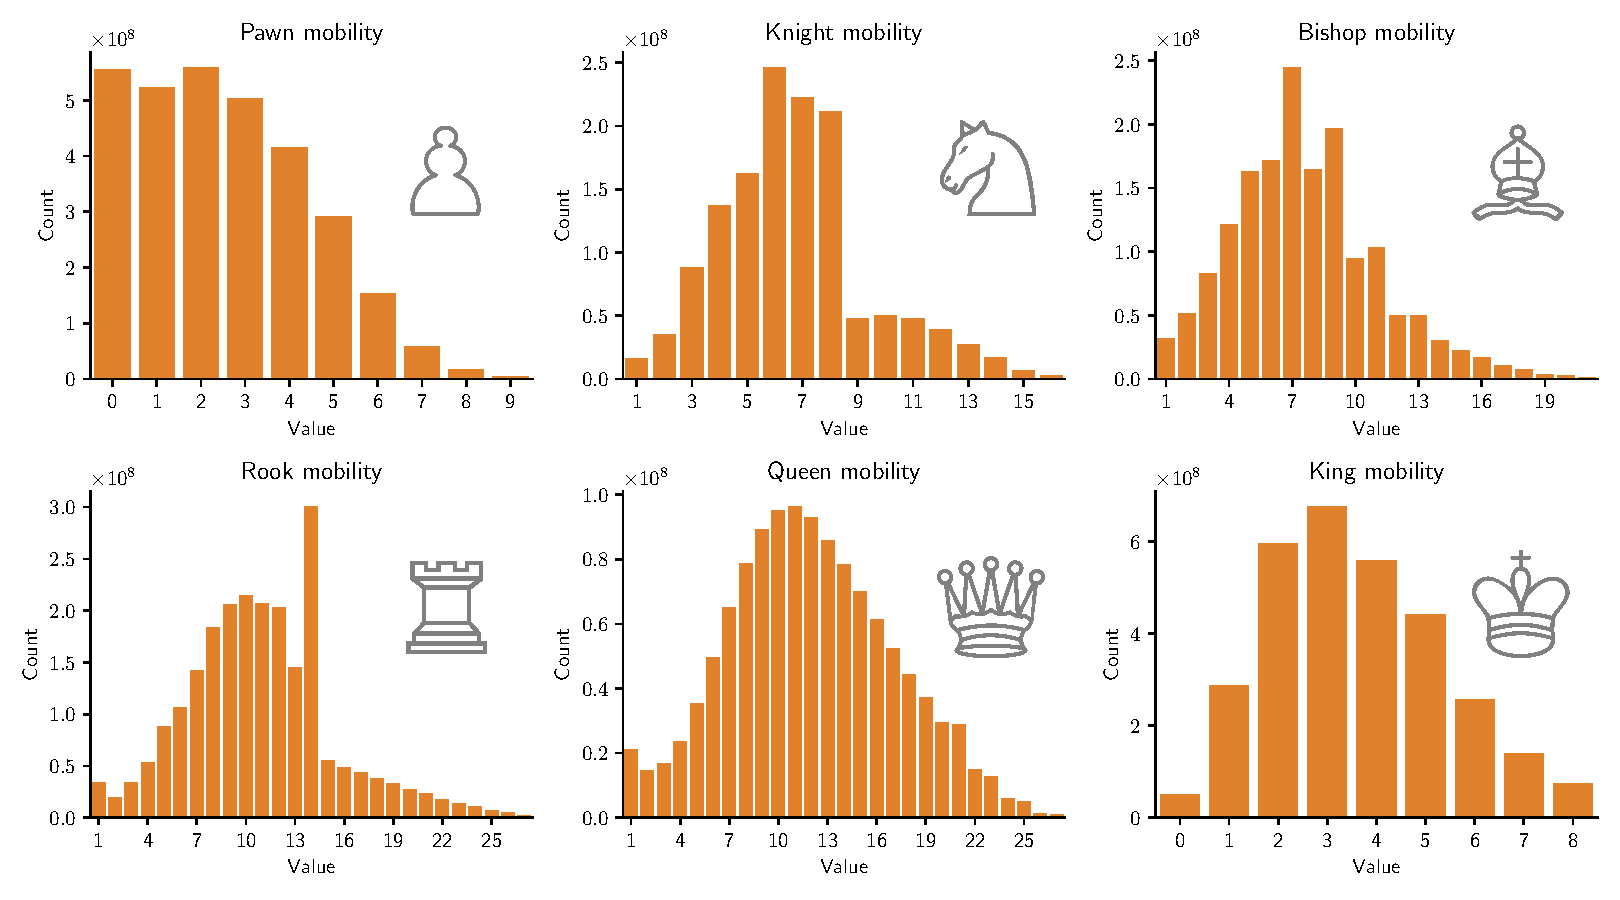
\includegraphics[width=0.95\textwidth]{../thesis/dynamic/output/mobility.pdf}}
\caption{Total mobility values for each piece on the board. Computed using 2 billion boards. The value 0 for the \symknight\ Knight, \symbishop\ Bishop, \symrook\ Rook, and \symqueen\ Queen has been excluded from the plot, as it is very common.}
\end{figure}
\end{frame}


\begin{frame}
\frametitle{Mobility: experimento}
\begin{table}
\centering
\begin{adjustbox}{max width=\textwidth}
\begin{tabular}{ccc}
\toprule
\bf Block name & \bf Definition & \bf Number of features \\
\toprule
MB & \makecell{
\vspace{0.2cm}
($\featureset{Squares} \times \featureset{Roles} \times \featureset{Colors})_P$ \\
P($\langle s, r, c \rangle$): there is a piece of role $r$\\ and color $c$ that \textbf{can move to} square $s$
} & 768 \\
\toprule
MC & \makecell{
\vspace{0.2cm}
$(\{0, 1, \hdots\} \times \featureset{Roles} \times \featureset{Colors})_{P}$\\
P($\langle m, r, c \rangle$): the value of mobility for\\
a piece of role $r$ and color $c$ is $m$
} & 206 \\
\bottomrule
\end{tabular}
\end{adjustbox}
\end{table}
Los feature sets a entrenar son: \featureset{All} $\oplus$ \featureset{MB} (1536 features) y \featureset{All} $\oplus$ \featureset{MC} (974 features).
\end{frame}

\begin{frame}
\frametitle{Mobility: resultados}
\begin{table}
\caption{Mobility encodings results}
\centering
\begin{tabular}{ccccc}
\toprule
\bf Feature set  & \bf \makecell{Number\\of features} & \makecell{\bf Val. loss\\\textit{min}} & \makecell{\bf Rating\\\textit{elo (rel. to \featureset{All})}} \\
\toprule
\featureset{All} (reference) & 768 & 0.003134 & \textbf{0.0} \\
\midrule
\featureset{All} $\oplus$ \featureset{MB} & 1536 & 0.002824 & -260.9 $\pm$ 5.4 \\
\midrule
\featureset{All} $\oplus$ \featureset{MC} & 974 & 0.003032 & -280.9 $\pm$ 5.6 \\
\bottomrule
\end{tabular}
\end{table}
\begin{itemize}
\item Las predicciones mejoran muy poco (el loss no se reduce tanto).
\item Por ende, el costo de las actualizar los features es más alto al beneficio que aportan. \pause
\item \featureset{MB} tiene más updates que \featureset{MC}, pero menor loss que compensa.
\end{itemize}
\end{frame}
